\justifying
\begin{problem}{1}
	Сила $F$ надає тілу масою $m_1$ прискорення $2 \dfrac{\text{м}}{\text{с}^2}$, а тілу масою $m_2$ -- прискорення $3 \dfrac{\text{м}}{\text{с}^2}$. Якого прискорення під дією тієї ж сили набудуть обидва тіла, коли їх з'єднати?
\end{problem}

\begin{problem}{2}
	Якісні питання:
	
	\begin{enumerate}
		\item Чому людині, яка стоїть у човні. який рухається, важко зберегти попереднє положення, коли човен зупиняється?
		
		\item Потяг рухається прямолінійною ділянкою шляху, на потяг діє сила тяги тепловоза, яка зрівноважується з силою тертя. Як рухається потяг? Як проявляється в цьому випадку закон інерції?
		
		\item На рис. наведено графік швидкості тіла. Що можно сказати про сили, які діють на це тіло?
		\begin{figure}[h!]
			\centering
			
			\begin{subfigure}{.4\textwidth}
				\begin{tikzpicture}
				\begin{axis}[xlabel = {$t$},
				ylabel = {$v, \text{м/с}$}]
				\addplot coordinates {
					(0,2) (2,2) (4,8) (6,8)
				};
				
				\end{axis}
				\end{tikzpicture}
			\caption{До задачі 4.2}
			\end{subfigure}
			\begin{subfigure}{.4\textwidth}
				\centering
				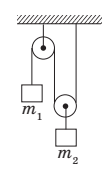
\includegraphics[width=0.5\linewidth]{class4/blocks}
				\caption{До задачі 4.11}
				\label{fig:blocks}
			\end{subfigure}			
			\caption{}
			\label{body}
		\end{figure}
	
		\item Який характер зміни рівнодіючої сил, які прикладені до автомобіля, графік якого наведений на попередньому рисунку
		
		\item Як буде рухатись ракета, якщо на неї діє постійна сила? постійно спадна сила?
	\end{enumerate}
\end{problem}

	\begin{problem}{3}
		Для того, щоб змінити свою вагу достатньо увійти в кабіну ліфта. Якиою, на Вашу думку, стане вага $P$ людини масою $m = 80$ кг в момент, коли швидкість ліфта напрямлена вгору і рівна $v = 1 \dfrac{\text{м}}{\text{с}}$, а прискорення напрямлено вниз і рівне $a = 1.8~\dfrac{\text{м}}{\text{с}^2}$
	\end{problem}

	\begin{problem}{4}
		Сила натягу кожної половини тятиви лука дорівнює $30$ Н, а кут між ними -- $120^{\circ}$. Яким буде початкове прискорення стріли лука, якщо її маса дорівнює $2.5$ кг?
	\end{problem}

	\begin{problem}{4}
		Через блок перекинули нитку, до кінців якої прикріплені тягарці, маса кожного з яких дорівнює $200 $г. Яку силу необхідно прикласти до одного з них, щоб тіла почали рухатись із прискоренням $0.5 \dfrac{\text{м}}{\text{с}^2}$ 
	\end{problem}

	\begin{problem}{5}
		На гладенькому столі лежать два бруски з масами $m_1 = 400$ г і $m_2 = 600$ г. До одного з них прикладено горизонтальну силу $F = 2$ Н. Визначте сили натягу $T$ нитки. якщо сила прикладена 
		\begin{enumerate}
			\item до першого бруска
			\item до другого бруска (самостійно)
		\end{enumerate}
	\end{problem}

	\begin{problem}{6}
		Тіло масою $m$ покоїться на горизонтальній поверхні в полі земного тяжіння. Коефіцієнт тертя між тілом та поверхнею -- $\mu$. До тіла прикладається сила $\vec{F}$ під кутом $\alpha$ до горизонту. Знайти прискорення, з яким рухається тіло під дією цієї сили.
	\end{problem}

	\begin{problem}{7}
		У вагоні потяга, який рухається зі швидкістю $v = 72 \dfrac{\text{км}}{\text{год}}$, зважують на пружунних вагах тіло масою $m = 5$ кг. Визначте показ $P$ вагів, коли потяг рухається по заокругленню радіусом $R = 400$ м.
	\end{problem}


\textbf{Задачі для самостійного розв'язання}



\begin{problem}{6}
	Яке прискорення нададуть дві сили $30$ Н та $40$ Н, прикладені до тіла. маса якого $50$ кг, під кутом $60^{\circ}$ одна до одної? Опір рухові дорівнює $21$ Н.
\end{problem}

\begin{problem}{4}
	Дві гирі масами $m_1 = 7$ та $m_2 = 11$ кг висять на кінцях нитки, яка перекинута через блок. Гирі спочатку знаходились на одній висоті. Через який час $t$ після початку руху більш легка гиря опинится на $10$ см вище за важку?
\end{problem}

\begin{problem}{7}
	Два грузи з масами $m_1$ та $m_2$, зв'язані легкою мотузкою, лежать на горизонтальній поверхні. Мотузка витримує силу натягу $T$. Коефіцієнт тертя між кожним грузом то поверхнею рівен $\mu$. З якою силою можно тягнути перший груз паралельно, щоб шнур не порвався? спочатку шнур не натягнутий. 
\end{problem}

\begin{problem}{8}
	Визначити прискорення тіл, маси яких $m_1$ та $m_2$, i силу натягу ниток в системі, зображеної на рис. Масою блоків і ниток, тертям знехтувати.
\end{problem}

\begin{problem}{9}
	Швидкісні пасажирскі ліфти рухаються зі швидкістю $v = 3.6 ~\dfrac{\text{м}}{\text{c}}$. Маса кабіни ліфта з пасажирами може досягати значення $m = 1500$ кг. Графік залежності змііни швидкості ліфта при підйомі зображений на рис. \ref{lift}
	
	Знайти силу натягу троса. який утримує кабіну на початку підйому, в середині та в кінці підйому.
	
	\begin{figure}[h!]
		\centering
		\begin{tikzpicture}
		\begin{axis}[xlabel = {$t$},
		ylabel = {$v, \text{м/с}$}]
		\addplot coordinates {
			(0,0)  (2,3.6) (10,3.6) (12,0)
		};
			
		\end{axis}
		\end{tikzpicture}
		\caption{}
		\label{lift}
	\end{figure}

\end{problem}

\begin{problem}{10}
	Згадаємо відому казку про лебедя, рака та щуку, в якій вони намагаються зрушити віз, але в них нічого не виходить. Як згодом виявилось, щука робила все для того. щоб віз не поїхав. Лебідь тягнув віз з силою $F_0$, рак тягнув віз  силою $F_1$ та щука тягнула з силою $F_2$. Сила. яку прикладав рак, була напрямлена під кутом $\alpha $ до вертикалі. Але він мимоволі змінював його значення. А підступна щука це помічала, і одразу змінювала кут $\beta$, під яким була напрямлена її сила так, щоб віз залишався в рівновазі. Знайдіть залежність $\beta(\alpha)$. За яких умов на сили можливий стан спокою для візка? (рисунок нарисовать)
	
	\begin{figure}[h!]
		\centering
		\begin{tikzpicture}
		\draw (0,0) -- (0,2) -- (4,2) -- (4,0) -- (0,0);
		
		\draw [dashed] (2,3) -- (2,-1);
		
		\draw [->, thick] (2,1) -- (-2, 1);
		\node [above] at (-2, 1) {$\vec{F}_0$};
		
		\draw [->, thick] (2,1) -- (3, 3);
		\node [above] at (3, 3) {$\vec{F}_1$};
		
		\draw [->, thick] (2,1) -- (4, -1);
		\node [above] at (4, -1) {$\vec{F}_2$};
		
		\node [right] at (1.8, 1.5) {$\alpha$};
		\node [right] at (1.8, 0.5) {$\beta$};
		
		
		\end{tikzpicture}
		\caption{До задачі \arabic{assigments}.\arabic{problems}}
		\label{fairytale}
	\end{figure}
\end{problem}